\section{Installation Guide}
	The most recent builds of RaceTrack for \textbf{macOS} and \textbf{Windows} (x64) can always be found on the GitHub repository (\url{https://github.zhaw.ch/PathFinder/PSIT3-FS20-IT18ta_WIN-Team5}) under the section \textit{Nightly Build}:
	\begin{figure}[H]
		\centering
		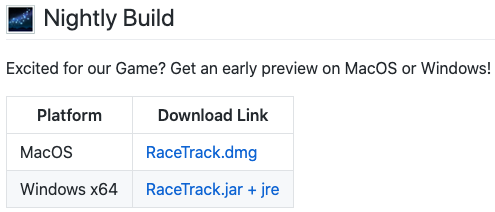
\includegraphics[width=10cm,keepaspectratio,center]{img/Implementation_Installation-Guide_Nightly-Build-Section.png}
		\caption{Documentation section in the GitHub repository}
	\end{figure}
	
	\subsection{macOS}
	\begin{enumerate}
		\item Execute the \textit{RaceTrack 1.0.dmg} file and copy \textit{RaceTrack.app} to your \textit{Applications} folder.
		\begin{figure}[H]
			\centering
			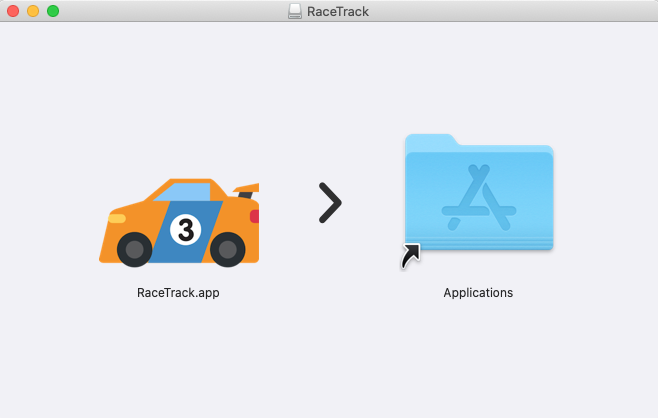
\includegraphics[width=8cm,keepaspectratio,center]{img/Implementation_Installation-Guide_macOS-1.png}
			\caption{Installation Guide for macOS: Copy to Applications folder}
		\end{figure}
		\item On the first time RaceTrack needs to be open via right-click, or else you'd not be able to skip the verification error message.
		\begin{figure}[H]
			\centering
			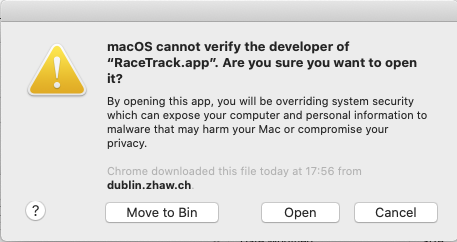
\includegraphics[width=8cm,keepaspectratio,center]{img/Implementation_Installation-Guide_macOS-3.png}
			\caption{Installation Guide for macOS: Skip verification error}
		\end{figure}
		\newpage
		\item After the first time, RaceTrack can be opened like any other application on your Mac.
		\begin{figure}[H]
			\centering
			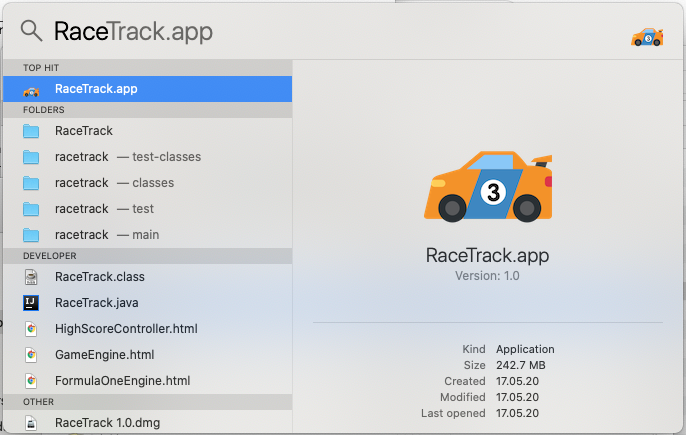
\includegraphics[width=8cm,keepaspectratio,center]{img/Implementation_Installation-Guide_macOS-4.png}
			\caption{Installation Guide for macOS: Start RaceTrack via Spotlight}
		\end{figure}
	\end{enumerate}

	\subsection{Windows}
	\begin{enumerate}
		\item Unzip the \textit{RaceTrack\_Windows64.zip} archive and execute \textit{RaceTrack.exe} in the just unzipped folder.
		\begin{figure}[H]
			\centering
			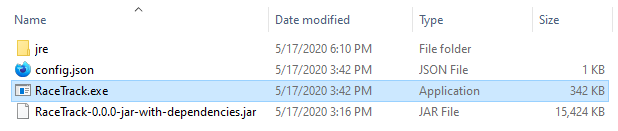
\includegraphics[width=10cm,keepaspectratio,center]{img/Implementation_Installation-Guide_Windows-1.png}
			\caption{Installation Guide for Windows: Unzip folder and execute .exe}
		\end{figure}
	\end{enumerate}
